\section{Bioimpedância Elétrica (BIA): Princípios, Métodos e Aplicações}

A bioimpedância elétrica (BIA) é um método indireto de avaliação da composição
corporal baseado nas propriedades elétricas dos tecidos biológicos. O princípio
fundamental da técnica está na diferença de condutividade elétrica entre tecidos
corporais, especialmente água, massa muscular e tecido adiposo. Tecidos com maior
conteúdo de água e eletrólitos apresentam menor resistência elétrica, enquanto o
tecido adiposo apresenta maior resistência.

A BIA mede parâmetros elétricos como resistência (R) e reatância (Xc), utilizados em
modelos matemáticos para estimativa de compartimentos corporais. Esses modelos podem
ser de frequência única, multifrequenciais ou espectroscópicos~\cite{kyle2004,lukaski1986}.

A técnica é muito usada em contextos clínicos, esportivos e epidemiológicos por ser
prática, barata e não invasiva. Sua precisão, porém, depende de fatores como
hidratação, alimentação recente, exercício físico e temperatura da pele, o que exige
protocolos de medição padronizados~\cite{espen2025,sossou2022}. Esses princípios estão
na base dos parâmetros fornecidos pela CF577BLE, analisada neste trabalho.

\subsection{Princípios físicos e modelagem da composição corporal}
\label{sec:principios}

A interpretação da BIA baseia-se na relação entre condutividade elétrica dos tecidos e
sua composição hídrica. A resistência elétrica corporal está inversamente relacionada
ao conteúdo de água corporal total.

A massa livre de gordura (\emph{Fat-Free Mass} --- FFM) é estimada por modelos
matemáticos baseados, em geral, na relação entre a altura ao quadrado e a impedância
elétrica corporal, conforme descrito na literatura clássica~\cite{kushner1992,kyle2004},
na forma da Equação~\ref{eq:ffm-classica}:

\equacao{eq:ffm-classica}{\mathrm{FFM} \propto \dfrac{\mathrm{Estatura}^2}{Z}}

\noindent onde $Z$ representa a impedância elétrica corporal. A partir da FFM,
derivam-se outras variáveis: a massa de gordura (peso total menos FFM), a água
corporal total (uma fração da FFM), a proteína corporal (aproximadamente 20\% a 25\%
da FFM) e a massa mineral (por modelos compostos).

O índice de massa muscular esquelética (SMI) é definido pela relação entre a massa
muscular esquelética e a estatura ao quadrado, conforme a Equação~\ref{eq:smi}:

\equacao{eq:smi}{\mathrm{SMI} = \dfrac{\mathrm{Massa\ muscular\ esquel\acute{e}tica}}{\mathrm{Estatura}^2}}

Massa livre de gordura, massa muscular esquelética e água corporal total estão na base
da maioria das métricas mostradas pelos dispositivos atuais de bioimpedância. Entender
os modelos matemáticos por trás dessas variáveis é necessário para interpretar
corretamente os resultados de equipamentos como a CF577BLE e dos sistemas
desenvolvidos neste trabalho.

\section{Tecnologias de Bioimpedância e Modelos de Estimativa Corporal}

O InBody 270S é uma das referências comerciais da bioimpedância segmentada
multifrequencial, usada em contextos clínicos, esportivos e de pesquisa~\cite{inbody2025}.

Esses aparelhos usam a análise direta segmentar multifrequencial (DSM-BIA), medindo
separadamente os cinco segmentos corporais (braços, pernas e tronco) em várias
frequências. O método chega a 15 medições de impedância, combinando três frequências
(20~kHz, 50~kHz e 100~kHz) em cada segmento. Isso separa a água intracelular da
extracelular e melhora a acurácia fisiológica das estimativas~\cite{besthealth2023,inbody2021}.

Ao contrário dos modelos empíricos tradicionais, esses sistemas dependem menos de
variáveis como idade e sexo e se apoiam mais em medições físicas diretas de cada
segmento. Os algoritmos, porém, são proprietários e pouco transparentes, o que limita
a reprodutibilidade científica~\cite{kyle2004}. Ainda assim, servem de referência para
entender os algoritmos usados em dispositivos domésticos.

O InBody 270S representa o estado da arte da bioimpedância segmentada multifrequencial,
mas dispositivos domésticos mais baratos vêm adotando conceitos parecidos no hardware e
no software. Por isso vale analisar a balança CF577BLE, usada como base experimental
deste trabalho~\cite{manualsplus2025}.

\subsection{Balanças de 8 eletrodos e análise segmentar}

As balanças de oito eletrodos avançam em relação aos modelos tradicionais: medem
tronco e membros separadamente, o que aumenta a precisão e permite interpretações mais
detalhadas para uso clínico e para aplicativos de saúde~\cite{manualsplus2025}.

Ao considerar a distribuição regional dos tecidos, o modelo ganha sensibilidade, o que
é útil principalmente em idosos, atletas e pessoas com obesidade. O princípio de
funcionamento baseia-se na medição da impedância segmentar, com diferenças regionais
associadas ao conteúdo hídrico e tecidual~\cite{lukaski1986}.

\subsection{Aplicações clínicas e uso da BIA na prática médica}

A bioimpedância elétrica é amplamente utilizada na prática clínica como ferramenta
auxiliar na avaliação da composição corporal e no acompanhamento de condições
relacionadas ao estado nutricional e metabólico. Entre suas principais aplicações
destacam-se o monitoramento nutricional de pacientes com sobrepeso, obesidade ou
desnutrição~\cite{espen2025}; a avaliação de risco metabólico e cardiovascular por
indicadores como percentual de gordura e gordura visceral; o acompanhamento clínico
longitudinal em doenças crônicas e reabilitação; e a promoção da saúde e a prevenção,
pela identificação precoce de alterações de risco.

Apesar da ampla aplicação, fatores como hidratação, alimentação recente, exercício
físico e temperatura corporal podem influenciar significativamente as medições,
exigindo interpretação clínica contextualizada~\cite{espen2025}.

\section{Funcionamento da Balança CF577BLE e Modelagem Computacional}

Dispositivos clínicos como o InBody 270S usam protocolos validados e hardware dedicado
para análise segmentar multifrequencial, enquanto dispositivos domésticos mais
acessíveis, como a CF577BLE, buscam reproduzir esses princípios com sensores
simplificados e algoritmos proprietários.

Vários dispositivos comerciais de origem asiática usam modelos algorítmicos inspirados
nos de equipamentos clínicos, como o algoritmo Body270 ou Body270S~\cite{besthealth2023},
aproximando-se do padrão técnico de sistemas como o InBody 270S.

A balança CF577BLE é um dispositivo de uso doméstico integrado ao ecossistema de
aplicativos como o Unique Health, associado a plataformas comerciais de origem chinesa
(Lefu/Tuya). O equipamento usa a bioimpedância elétrica para estimar a composição
corporal, com transmissão de dados por Bluetooth Low Energy (BLE) e Wi-Fi.

O aparelho aplica uma corrente elétrica de baixa intensidade por eletrodos de contato
plantar e processa os dados com algoritmos proprietários. A análise segmentar
multifrequencial mede a impedância em diferentes regiões do corpo, incluindo braços,
pernas e tronco.

Como em equipamentos clínicos mais avançados, o sistema mede cinco segmentos corporais
(braço direito, braço esquerdo, tronco, perna direita e perna esquerda) e pode chegar a
15 medições de impedância, combinando três frequências (20~kHz, 50~kHz e 100~kHz). Isso
permite estimar de forma indireta a água intracelular e a extracelular, segundo a
documentação técnica do algoritmo Body270~\cite{besthealth2023}, e aumenta a resolução
da distribuição hídrica corporal. Essa combinação de múltiplas frequências com análise
segmentar é a mesma usada em aparelhos clínicos como o InBody 270S, o que mostra a
proximidade técnica entre equipamentos profissionais e soluções comerciais com
algoritmos proprietários.

O modelo de resistências segmentares adotado segue as representações fisiológicas usadas
em sistemas de bioimpedância segmentar e reproduz a distribuição desigual de fluidos do
corpo, como na Figura~\ref{fig:resistencias}: membros superiores esquerdo e direito com
cerca de 300~$\Omega$, tronco com cerca de 24~$\Omega$ e membros inferiores esquerdo e
direito com cerca de 240~$\Omega$. O tronco é a região de menor resistência, pelo maior
volume de fluidos e tecidos condutores, enquanto os membros têm resistência relativa
maior.

\begin{figure}[!ht]
    \centering
    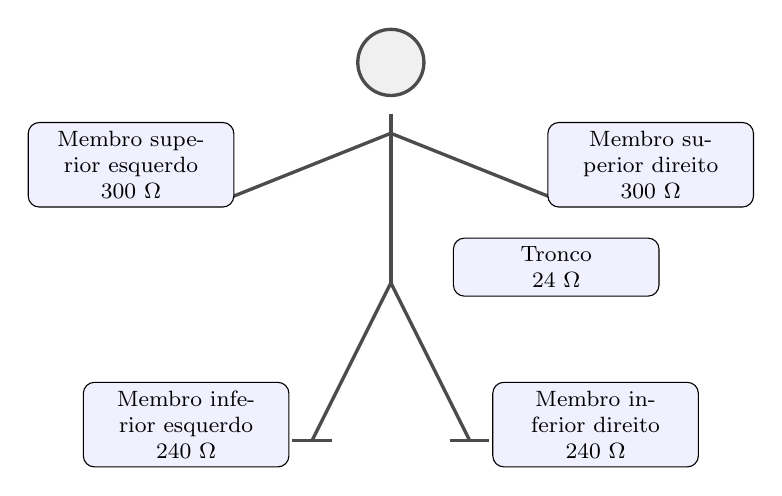
\begin{tikzpicture}[
        seg/.style={very thick, gray!60!black},
        lab/.style={draw, rounded corners, fill=blue!6, font=\footnotesize,
                    align=center, inner sep=3pt, text width=2.4cm},
    ]
        % cabeça
        \draw[seg, fill=gray!12] (0,4.5) circle (0.42);
        % tronco
        \coordinate (ombro)   at (0,3.85);
        \coordinate (quadril) at (0,1.7);
        \draw[seg] (ombro) -- (quadril);
        % braços
        \draw[seg] (0,3.6) -- (-2,2.8);
        \draw[seg] (0,3.6) -- (2,2.8);
        % pernas
        \draw[seg] (quadril) -- (-1,-0.3);
        \draw[seg] (quadril) -- (1,-0.3);
        % pés
        \draw[seg] (-1.25,-0.3) -- (-0.75,-0.3);
        \draw[seg] (0.75,-0.3) -- (1.25,-0.3);
        % rótulos
        \node[lab] at (-3.3,3.2)  {Membro superior esquerdo\\ 300~$\Omega$};
        \node[lab] at (3.3,3.2)   {Membro superior direito\\ 300~$\Omega$};
        \node[lab] at (2.1,1.9)   {Tronco\\ 24~$\Omega$};
        \node[lab] at (-2.6,-0.1) {Membro inferior esquerdo\\ 240~$\Omega$};
        \node[lab] at (2.6,-0.1)  {Membro inferior direito\\ 240~$\Omega$};
    \end{tikzpicture}
    \caption{Modelo de resistências segmentares do corpo humano utilizado na CF577BLE. O
    tronco tem a menor resistência, pelo maior volume de fluidos e tecidos condutores,
    enquanto os membros apresentam resistência relativa maior.}
    \label{fig:resistencias}
\end{figure}

Os dados são processados por um algoritmo proprietário, em geral chamado Body270 ou
Body270S, que usa um modelo de quatro compartimentos corporais (gordura, água, proteína
e minerais). É um avanço sobre os modelos clássicos de dois compartimentos e permite
estimativas mais detalhadas. Diferentemente das equações clássicas da literatura, como
os modelos de Lukaski ou Jaffé, o algoritmo Body270 não usa fórmulas explícitas do tipo
$\mathrm{Estatura}^2/Z$, mas regressões estatísticas multivariadas baseadas em dados
populacionais, integrando a impedância segmentar com variáveis antropométricas como
peso, altura, idade e sexo.

Pelo aplicativo, a CF577BLE fornece mais de 50 métricas, entre elas: parâmetros básicos
(peso, IMC e percentual de gordura corporal); composição corporal (massa muscular, massa
de gordura, massa magra, massa óssea, proteínas e água corporal); indicadores metabólicos
(taxa metabólica basal e ingestão calórica recomendada); análise segmentar (distribuição
de massa muscular e gordura por membros e tronco); indicadores de risco (gordura
visceral, gordura subcutânea e nível de obesidade); indicadores adicionais (idade
corporal, pontuação de saúde e tipo físico); e controle corporal (peso ideal estimado,
controle de gordura e controle muscular).

Apesar do volume de informações, o algoritmo foi projetado para avaliação de bem-estar e
monitoramento corporal, não para diagnóstico clínico. A própria documentação técnica
indica que os resultados são indicadores de referência (nível \emph{wellness}), e não
medidas médicas precisas. Além disso, os parâmetros de classificação podem variar
conforme a população de referência: limites de IMC e de percentual de gordura em
populações asiáticas tendem a ser mais restritivos do que os adotados em diretrizes
brasileiras e internacionais, o que pode afetar a interpretação.

Os dados aparecem no aplicativo em formato numérico e gráfico, com histórico de medições.
Diferentemente de equipamentos clínicos como o InBody 270S, a CF577BLE não fornece um
relatório estruturado com interpretação detalhada, limitando-se a classificações
genéricas. Embora use conceitos avançados de bioimpedância, como análise segmentar
multifrequencial e modelo de quatro compartimentos, a principal limitação do dispositivo
está no algoritmo proprietário, na falta de transparência metodológica e na ausência de
validação clínica explícita.

Essa limitação justifica sistemas complementares que interpretem os dados de forma
contextualizada e personalizada. É essa a proposta central do trabalho: usar
inteligência artificial para transformar as métricas brutas em informações úteis e
compreensíveis para o usuário. Não foram identificados estudos amplamente publicados de
validação cruzada do algoritmo Body270 com métodos de referência como o DXA, o que limita
a avaliação independente de sua acurácia. Uma comparação resumida entre a CF577BLE, o
algoritmo Body270 e o InBody 270S é apresentada no Anexo~A.

\section{Limitações da BIA e Comparação com Métodos de Referência}

Apesar da ampla utilização da BIA, diversos estudos demonstram vieses sistemáticos
quando ela é comparada à absorciometria por dupla emissão de raios X (DXA), considerada
padrão-ouro para avaliação da composição corporal~\cite{heymsfield2005}.

Em estudo com adultos e idosos brasileiros, observou-se alta correlação entre BIA e DXA
($r \approx 0{,}97$), mas com diferenças sistemáticas relevantes: a BIA superestimou a
massa livre de gordura (FFM) em cerca de 3,1~kg ($+7{,}2\%$) e subestimou a massa de
gordura em cerca de 2,9~kg ($-13{,}0\%$)~\cite{wahrlich2026}. Esses achados indicam vieses
estruturais associados a equações proprietárias calibradas em populações específicas.

Para mitigar esse erro, os autores propõem a equação de calibração da
Equação~\ref{eq:calibracao}:

\equacao{eq:calibracao}{\mathrm{DXA}_{\mathrm{FFM}} = 0{,}94420 \cdot \mathrm{BIA}_{\mathrm{FFM}} - (0{,}01128 \cdot \mathrm{idade}) + 0{,}20516}

Além disso, foi desenvolvido um modelo multivariado para estimativa direta da FFM,
apresentado na Equação~\ref{eq:ffm-wahrlich}:

\equacao{eq:ffm-wahrlich}{\begin{aligned}\mathrm{FFM}\,(\mathrm{kg}) ={}& (\mathrm{sexo} \cdot 4{,}1797) + (\mathrm{estatura} \cdot 0{,}1062) + (\mathrm{RI} \cdot 0{,}5289) \\ &+ (\mathrm{massa} \cdot 0{,}1797) - (\mathrm{idade} \cdot 0{,}0705) - 5{,}4286\end{aligned}}

Esses modelos reforçam que, embora a BIA tenha alta correlação com o DXA, sua acurácia
depende fortemente da população de calibração, sendo necessária adaptação local. O viés
associado à população de calibração mostra que é preciso adaptar localmente os modelos:
dispositivos domésticos, em geral calibrados com bases asiáticas ou norte-americanas,
podem apresentar diferenças adicionais em brasileiros. Por isso, estudos de ajuste
experimental e calibração indireta ajudam a tornar esses dispositivos mais aplicáveis no
contexto nacional, sobretudo quando combinados com modelos que integram variáveis
antropométricas, impedância segmentar e regressões da literatura.

Além do viés das equações, há variações ligadas ao estado fisiológico do momento.
Hidratação, exercício recente e alimentação podem alterar a impedância medida sem que a
composição corporal tenha mudado de fato. Isso pede métodos computacionais que
identifiquem e compensem em parte esses fatores de confusão, tema tratado neste trabalho
pela combinação de bioimpedância, coleta de contexto e inteligência artificial. Vale
lembrar que correlação alta entre métodos não significa concordância clínica alta: um
aparelho pode ter correlação forte com um método de referência e ainda manter diferenças
sistemáticas em nível individual. Por isso, o trabalho não pretende validar clinicamente
a bioimpedância como método diagnóstico, e sim criar mecanismos para interpretar,
contextualizar e acompanhar os dados do equipamento ao longo do tempo.

\subsection{Limitações inerentes aos algoritmos proprietários}

A bioimpedância segmentar multifrequencial melhorou a estimativa da composição corporal,
mas os algoritmos dos fabricantes continuam, em boa parte, proprietários. Por isso, os
cálculos exatos que transformam as medições elétricas em parâmetros fisiológicos não são
totalmente abertos à comunidade científica. Essa limitação dificulta a reprodutibilidade
e a comparação entre equipamentos, e parte das equações pode ter sido calibrada em
populações específicas, o que introduz vieses em grupos com características distintas.

Por isso, os resultados da CF577BLE devem ser lidos como estimativas fisiológicas úteis
para acompanhamento ao longo do tempo e observação de tendências, e não como equivalentes
a métodos de referência clínica, como o DXA.

\section{Comparação entre dispositivos e justificativa da escolha da CF577BLE}

Dispositivos de bioimpedância podem ser classificados em duas categorias principais:
equipamentos de uso clínico ou de pesquisa e dispositivos domésticos de monitoramento.
Equipamentos como a Tanita BC-418~\cite{tanita} têm maior validação empírica e padronização
metodológica, sendo muito usados em estudos comparativos com o DXA, ainda que também
apresentem viés dependente da população~\cite{kyle2004}. Dispositivos domésticos como a
CF577BLE usam modelos mais simples e menos específicos por população, o que aumenta a
variabilidade das estimativas e reduz a confiabilidade individual.

A CF577BLE foi escolhida neste estudo pela análise segmentar com oito eletrodos, pela
conectividade com aplicativos e pela variedade de parâmetros fisiológicos, o que a torna
adequada para integrar sistemas de interpretação da composição corporal. A escolha
atende ao objetivo do trabalho: desenvolver um aplicativo que interprete os dados da
balança em linguagem acessível, ofereça recomendações personalizadas e acompanhe o
progresso do usuário, indo além do simples registro de números.

\section{Modelos de Linguagem para Saúde: de LLMs a SLMs}

O uso de modelos de linguagem (\emph{Large Language Models} --- LLMs, como GPT e Gemini)
cresceu na saúde digital, sobretudo em triagem, apoio à decisão e interpretação de dados.
Mas LLMs generalistas têm limitações em cenários clínicos: alto custo computacional,
dependência de nuvens públicas, consumo elevado de energia e riscos à privacidade do
paciente. Essa dependência de infraestrutura externa contraria princípios de
\emph{privacy-preserving AI}, sobretudo diante da LGPD e das diretrizes internacionais de
ética digital em saúde.

Em resposta, cresceu o interesse pelos \emph{Small Language Models} (SLMs), modelos
menores e eficientes, que podem ser treinados localmente e rodar com baixo custo
computacional. A literatura recente situa esse movimento na chamada \emph{Green AI}, que
busca sistemas de IA com menor consumo de energia e menor impacto ambiental sem perder
desempenho em tarefas específicas~\cite{schwartz2020,hooker2021}.

Embora LLMs também permitam \emph{fine-tuning} e especialização, este trabalho opta por
modelos abertos, gratuitos e executáveis localmente. Essa escolha reduz a dependência de
serviços comerciais de inferência, elimina custos recorrentes de APIs proprietárias e dá
mais controle sobre o armazenamento e o processamento das informações. A execução local
reduz o risco de compartilhar dados sensíveis com servidores externos e atende a
requisitos de privacidade, auditabilidade e transparência, importantes em saúde. Modelos
menores também exigem menos recursos de computação e energia, o que facilita a adoção em
ambientes acadêmicos e institucionais.

A adoção de SLMs neste projeto fundamenta-se em três pilares: privacidade e soberania dos
dados dos usuários; eficiência energética e computacional; e especialização para a
interpretação da composição corporal e da bioimpedância. Por essas razões, o \sintonia\
adota SLMs.

Para adaptar modelos de linguagem a domínios específicos, há diferentes estratégias, como
\emph{fine-tuning}, recuperação de conhecimento externo (RAG), engenharia de \emph{prompt}
e regras de interpretação. Neste trabalho optou-se por regras especializadas e engenharia
de \emph{prompt}, sem treinamento adicional do modelo. Essas técnicas permitem construir
assistentes especializados na interpretação da composição corporal, que rodam localmente e
consomem poucos recursos.

\subsection{Dados Sintéticos em Aplicações de Saúde}

O treinamento de modelos de IA em saúde enfrenta desafios de disponibilidade de dados,
privacidade e conformidade regulatória. Como alternativa, cresce o uso de dados
sintéticos, gerados artificialmente para preservar características estatísticas dos dados
reais sem expor informações pessoais. Estudos recentes mostram que conjuntos sintéticos
podem ser usados para treinamento, validação e teste de modelos de aprendizado de máquina
em diversos cenários clínicos, reduzindo riscos de privacidade e ampliando a
disponibilidade de amostras~\cite{gonzalez2023}.

Em sistemas de composição corporal, dados sintéticos podem complementar bases reais de
bioimpedância durante o desenvolvimento e a avaliação dos modelos. O uso pede cautela:
dados artificiais nem sempre reproduzem a variabilidade fisiológica real e podem carregar
vieses do processo de geração. Por isso, sua aplicação deve vir acompanhada de validação
que confirme a coerência com os fenômenos biológicos modelados.

\section{Metabolismo Basal (TMB/BMR): Fundamentos, Cálculo e Relevância Clínica}

A Taxa de Metabolismo Basal (TMB) é o gasto energético mínimo para manter as funções
vitais em repouso. É influenciada por idade, sexo, fatores hormonais, nível de atividade
física e, sobretudo, pela quantidade de massa magra (músculos, órgãos e ossos)~\cite{cunningham1991}.
A TMB responde pela maior parcela do gasto energético diário, entre 60\% e 75\%.

Várias equações estimam a TMB na clínica: Harris--Benedict, Mifflin--St Jeor,
Katch--McArdle, entre outras~\cite{wenna2023}. Estudos recentes mostram que essas fórmulas,
embora difundidas, apresentam erros relevantes em pessoas muito musculosas, obesas,
idosas ou com composições atípicas, porque foram derivadas de amostras específicas e não
refletem a heterogeneidade corporal atual~\cite{franks2023,henry2005}.

Equações baseadas só em peso e altura, por exemplo, tendem a superestimar a TMB de pessoas
obesas e a subestimar a de atletas com muita massa magra. A de Katch--McArdle, que usa a
massa magra estimada, é mais precisa, mas depende da qualidade da medida, na prática
obtida por bioimpedância. Combinar BIA segmentada com a TMB estimada melhora a
interpretação da composição corporal no emagrecimento, em atletas e em tratamentos
metabólicos.

\section{Emagrecimento Saudável}

O emagrecimento sustentável depende de déficit calórico moderado, manutenção da massa
magra e hábitos consistentes. Dietas muito restritivas tendem a derrubar a TMB, causar
perda muscular e gerar ciclos de recuperação de peso. Profissionais como Márcio Atalla,
especialista em treinamento de atletas de alto nível~\cite{atalla2025}, reforçam o papel
de atividade física regular, alimentação equilibrada e acompanhamento contínuo.

\subsection{Preservação da massa magra e exercícios}

Musculação, exercício aeróbico e ingestão adequada de proteína ajudam a reduzir a perda
de massa magra durante o emagrecimento. Com isso, a TMB se mantém mais estável, há menos
platôs metabólicos e menor risco de recuperar o peso perdido. No conjunto, é um
emagrecimento mais sustentável, que preserva a musculatura e ajuda a manter o peso no
longo prazo.

\subsection{Métricas apresentadas por wearables (relógios e pulseiras)}

Relógios inteligentes e pulseiras esportivas estimam o gasto energético combinando
sensores de movimento, frequência cardíaca e algoritmos proprietários. Embora úteis para
o monitoramento contínuo da atividade física, estudos recentes indicam que as estimativas
de gasto energético ainda têm limitações relevantes frente a métodos de referência. Os
erros variam conforme o dispositivo, o tipo e a intensidade da atividade e os algoritmos,
podendo superar 30\% em certas condições~\cite{germini2022,doherty2024}. Recomenda-se, por
isso, interpretar essas estimativas como indicadores relativos de acompanhamento, e não
como medidas absolutas.

\subsection{Agonistas de GLP-1 (``canetas para emagrecer'')}

Medicamentos como semaglutida, tirzepatida e outros agonistas de GLP-1 têm eficácia
comprovada para perda de peso, mas parte significativa da massa perdida pode incluir massa
magra, o que reforça a necessidade de monitoramento frequente da composição
corporal~\cite{wilding2021}. O uso exige acompanhamento médico, sobretudo pelo risco de
perda desproporcional de massa magra, por efeitos gastrointestinais, pelo risco de ganho
de peso após a interrupção e pelo impacto psicológico e comportamental. Quem usa esses
medicamentos pode se beneficiar do monitoramento frequente da composição corporal, o que
reforça a utilidade de soluções como o \sintonia.

\section{Integração BIA + TMB + IA (SLM): Potencial para Interpretação Personalizada}

Integrar dados de BIA segmentada, estimativas de TMB e histórico longitudinal de saúde
permite gerar análises personalizadas relevantes para usuários leigos e profissionais. Um
SLM ajustado para esse domínio pode traduzir números técnicos (por exemplo, massa magra
dos membros inferiores, gordura visceral e idade corporal) em mensagens claras, como
``sua massa muscular em braços e pernas está abaixo da média, o que reduz sua taxa
metabólica basal'' ou ``houve redução de gordura visceral, o que melhora sua saúde
metabólica''.

Essa camada de interpretação ajuda o usuário a entender os dados, reduz erros de
autoavaliação e apoia o autocuidado. Como roda localmente, o SLM mantém os dados sensíveis
privados. Combinar BIA, TMB e SLM cria um acompanhamento de saúde personalizado, de baixo
custo e alinhado às práticas atuais de saúde digital e IA responsável.

\section{Sistemas Inteligentes para Interpretação da Composição Corporal}

Os aparelhos modernos de bioimpedância fornecem dezenas de indicadores, mas interpretá-los
em conjunto ainda é difícil para quem não tem formação técnica. Percentual de gordura,
massa muscular, água corporal, metabolismo basal e gordura visceral costumam aparecer
isolados, o que dificulta entender o quadro geral de saúde. A literatura recente de saúde
digital indica que sistemas de IA podem funcionar como camada entre os dados fisiológicos
e o usuário, traduzindo métricas complexas em orientações compreensíveis e
contextualizadas.

O \sintonia\ propõe uma arquitetura integrada: aquisição automática dos dados de
bioimpedância, coleta do contexto fisiológico por anamnese, análise por modelos de
linguagem especializados e acompanhamento ao longo do tempo. A ideia é unir os benefícios
da bioimpedância segmentada à IA para entregar interpretações personalizadas e apoiar o
monitoramento da saúde.

\section{Aspectos Éticos e IA Responsável em Sistemas de Saúde Digital}

Aplicações de IA em saúde exigem cuidados com privacidade, transparência, explicabilidade
e responsabilidade das recomendações. Sistemas que geram interpretações sobre indicadores
fisiológicos devem evitar conclusões diagnósticas automáticas e apresentar suas análises
como informações de apoio. Em linha com isso, o \sintonia\ adota princípios de IA
responsável: coleta mínima de dados, anonimização do que é armazenado, possibilidade de
rodar os modelos de linguagem localmente e respostas de caráter educacional e informativo.
As recomendações do sistema não substituem avaliação médica, nutricional ou de educação
física.

A revisão mostra que a bioimpedância elétrica é muito usada para estimar a composição
corporal, embora tenha limitações metodológicas, operacionais e populacionais. Os
dispositivos domésticos atuais já trazem tecnologia segmentar e multifrequencial e geram
muita informação fisiológica, mas interpretá-la ainda é difícil para o usuário leigo. Ao
mesmo tempo, os \emph{Small Language Models} permitem sistemas especializados com menor
custo computacional e mais privacidade. É nesse cruzamento que o trabalho se situa:
integrar bioimpedância, modelagem computacional e IA para interpretar as métricas
corporais de forma personalizada e ajudar a entender os resultados da CF577BLE.
